\documentclass{article}
\usepackage{graphicx} % Required for inserting images
\usepackage[margin=1.0in]{geometry}
\usepackage{float}
\usepackage{hyperref}
\usepackage{listings}

\linespread{1}
\setlength{\parindent}{0pt} % Disable paragraph indentation

\title{CPEN 333 Final Project : Part I (Multithreaded Game)}
\author{Group G6 : Muntakim Rahman and Tomaz Zlindra}
\date{December 6th, 2024}

\begin{document}

\maketitle

\section{Requirements and Constraints}

We were provided the template with skeleton code (i.e. classes, methods with docstrings) for the implementation of the Snake Game.
The key design structure entailed the following requirement: \\

\textbf{Use \texttt{Queue.queue} module to ensure multi-producer, multi-consumer achieves synchronization between threads} (i.e. add \texttt{dict} items to the queue for "\texttt{game\_over}", "\texttt{score}", "\texttt{prey}", "\texttt{move}").

\section{Implementation}

We were provided fully functional \texttt{Gui}, \texttt{QueueHandler} classes with a \texttt{gameQueue} instance of the standard \texttt{Python Queue}' class.
Our task was to implement the following methods of the \texttt{Game} class.

\begin{itemize}
    \item \texttt{superloop()}
    \item \texttt{move()}
    \item \texttt{calculateNewCoordinates()}
    \item \texttt{isGameOver(snakeCoordinates:tuple)}
    \item \texttt{createNewPrey()}
\end{itemize}

\subsection{UML Relationships}

We utilized the template data fields and methods to program a responsive and thread-safe Snake Game, as shown in the UML Relationships in Figure \ref{fig:Part1_ClassDiagrams}. \\

These enabled the program to update the game state via the \texttt{Game} class and display this to the user via the \texttt{Tkinter} widgets in the \texttt{Gui} class.

\begin{figure}[H]
    \centering
     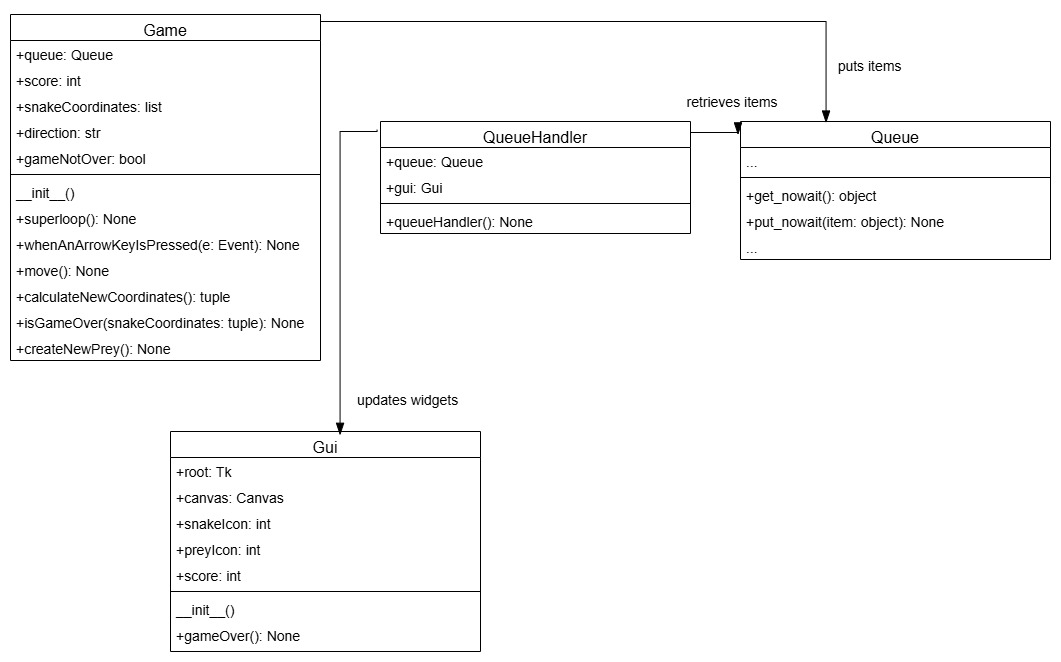
\includegraphics[width=0.8\textwidth]{../Part_1_ClassDiagrams.jpg}
     \caption{Part 1 - UML Relationships}
     \label{fig:Part1_ClassDiagrams}
 \end{figure}

\subsection{Gameplay}

The game is played with the \texttt{superloop()} method in a \texttt{daemonic thread}, until the \texttt{game.gameNotOver} data field is read as \texttt{False}.
A conditional loop in the \texttt{superloop()} method calls the \texttt{move()} method
every \texttt{SPEED} \textit{ms} to perform the following actions:

\begin{enumerate}
    \item Determine the new head coordinates of the snake (i.e. based on current direction). (See \nameref{sec:New_Snake_Coordinates}.)
    \item If the prey has been captured: (See \nameref{sec:Prey_Capture}.)
    \begin{enumerate}
        \item Append the head to the \texttt{game.snakeCoordinates} data field (i.e. increase its length by \texttt{SNAKE\_ICON\_WIDTH}).
        \item Increment the score and \textbf{put this in the \texttt{gameQueue}}.
        \item Randomly pick a valid (\textit{x}, \textit{y}) coordinate pair for the new prey. \textbf{Put this in the \texttt{gameQueue}.} (See \nameref{sec:Prey_Generation}.)
    \end{enumerate}
    \item If the prey has not been captured :
    \begin{enumerate}
        \item Shift the the \texttt{game.snakeCoordinates} data field forward by one item (i.e. to simulate movement).
    \end{enumerate}
    \item If the snake has hit itself / the wall : update the \texttt{game.gameNotOver} data field to be \texttt{False}. \textbf{Put this in the \texttt{gameQueue}.} (See \nameref{sec:Game_Over}.)
    \item\textbf{Put the new coordinates list (i.e. \texttt{game.snakeCoordinates} data field) in the \texttt{gameQueue}.}
\end{enumerate}

\textbf{Note that items are put in the \texttt{gameQueue} with the \texttt{put\_nowait(item)} method from the \texttt{Queue} class since it is non-blocking.} \\

Let's look at a few of the implemented methods in detail.

\subsubsection{\texttt{calculateNewCoordinates()}}\label{sec:New_Snake_Coordinates}
A conditional statement  method reads the current value of the \texttt{game.direction} data field to
shift the head coordinates in the respective direction. This is computed as an addition/substraction of the relevant \textit{x} or \textit{y} coordinate by \texttt{SNAKE\_ICON\_WIDTH}.

\subsubsection{\texttt{createNewPrey()}}\label{sec:Prey_Generation}
We used the \texttt{randint()} function from the \texttt{random} library to generate an integer for the (\textit{x}, \textit{y}) coordinate pair. This follows the calculation
in the provided docstring to consider coordinates a \texttt{THRESHOLD} margin away from the edge of the \texttt{Tkinter Canvas}. We subtracted/added half of the \texttt{PREY\_ICON\_WIDTH}
in either direction and put these edge coordinates into the \texttt{gameQueue}. \\

\textit{Note that the new prey can spawn in the same coordinates as the snake body / head. This is by design (i.e. for simplicity) and may be considered a capture based on the capture logic below.}

\subsubsection{\texttt{isCaptured(snakeCoordinates: tuple, preyCoordinates: list)}}\label{sec:Prey_Capture}

We designed the logic for capturing the prey to account for different sizes of both the prey and snake head. This was captured by the inner function in the \texttt{move} method. \\

We determined the edge coordinates of both the prey and the snake's head. We then checked whether any point of the snake's head
fell within the prey's boundaries (and vice-versa), as illustrated in figure \ref{fig:PreyCapture}. \\

\textit{Note that the \texttt{Canvas.coords(gui.preyIcon)} method was used to retrieve the x0, y0, x1, y1 points.}

\begin{figure}[H]
   \centering
    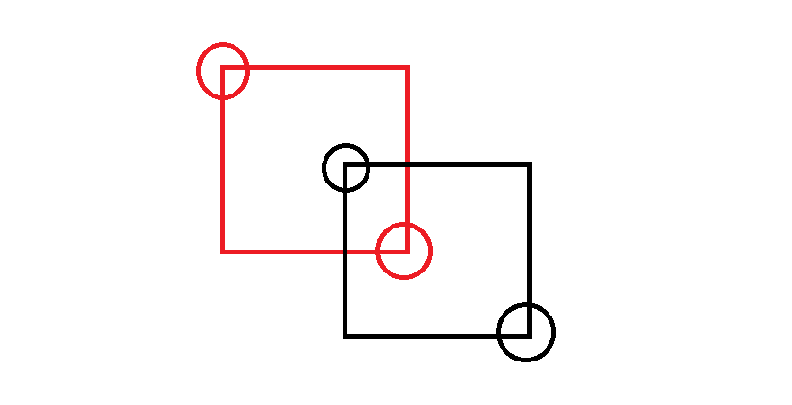
\includegraphics[width=0.6\textwidth]{../PreyCapture.png}
    \caption{Prey Capture Criteria : Edge Coordinate Of Prey/Snake Must Be Contained}
    \label{fig:PreyCapture}
\end{figure}

Since \texttt{Canvas.create\_line(...)} renders a \textit{1-D} widget
for the \texttt{gui} instance, we considered a \textit{radius} of half the \texttt{SNAKE\_ICON\_WIDTH} along the relevant \textit{x} or \textit{y} coordinate, depending on the current value of
the \texttt{game.direction} data field. This is similar to the logic in the \texttt{createNewPrey()} method.

\subsubsection{isGameOver(self, snakeCoordinates: tuple)}\label{sec:Game_Over}
The game ends once either of the following has occurred:
\begin{itemize}
    \item snake's head exits the canvas bounds
    \item snake's head hits its body (i.e. head and body have same (\textit{x}, \textit{y}) coordinate pair)
\end{itemize}

\end{document}
